\documentclass{article}
\usepackage{graphicx} % Required for inserting images
\usepackage{enumitem}
\usepackage{amsmath}
\usepackage{textgreek}
\usepackage{listings}
\usepackage{hyperref}
% Adjust page margins
\usepackage[margin=1in]{geometry}
\usepackage{titlesec}
\setlength{\leftmargin}{1.5in}
% Custom formatting for chapter titles
\titleformat{\chapter}[block]
  {\fontsize{18pt}{0pt}\selectfont\bfseries}
  {\thechapter}
  {1em}
  {\MakeUppercase}
\usepackage{titlesec}
\usepackage{float} % for H specifier



\begin{document}

\begin{figure}
    \centering
    
\includegraphics[width=0.7\linewidth]{logoENCS.jpeg}
    \label{fig:example}
\end{figure}

\begin{center}
{\fontsize{16pt}{0pt}\selectfont \textbf{Documentation of Metricstics}} \\
  \vspace{20pt}
  {\fontsize{14pt}{0pt}\selectfont \textbf{Submitted by}}
  \\
\vspace{30pt}


\begin{large}
\begin{tabular}{ c c c }
 \textbf{Het Jatin Dalal}& \textbf{40200513} \\ 
  \textbf{Abderraouf Drine}& \textbf{40225137}  \\  
  \textbf{Chae Dickie-Clark} & \textbf{23345718}  \\ 
  \textbf{Protim Ghosh} & \textbf{40185075} \\
  \textbf{Abhishek Deswal} & \textbf{40220734} \\
\end{tabular}
\end{large}
\\
\vspace{100pt}
{\fontsize{14pt}{0pt}\selectfont \textbf{SOFTWARE MEASUREMENT}}\\
\vspace{20pt}
{\fontsize{14pt}{0pt}\selectfont \textbf{SOEN 6611}}
\\
\vspace{20pt}
{\fontsize{14pt}{0pt}\selectfont \textbf{Group D}}
\\
\vspace{130pt}
{\fontsize{14pt}{0pt}\selectfont \textbf{Fall 2023}}
\end{center}

\section{Installation}
    Metricstics can be installed by cloning the repository from \url{https://github.com/MajorTreble/Metricstics}. It requires Python 3.8+ to run.\\
    \\
Install the requirements using
\begin{lstlisting}
pip install -r requirements.txt
\end{lstlisting}

From the root folder, run the app using

\begin{lstlisting}
python metricstics/src/app.py
\end{lstlisting}

\section{Usage}

\begin{enumerate}
    \item \textbf{Read Data:} Following screenshot shows how to use read data functionality along with the results. On pressing this button, the system will read data from its database(File in our case) and after that user can press other buttons(functionality) as per need to obtain different results
    \begin{figure}[h]
        \centering
        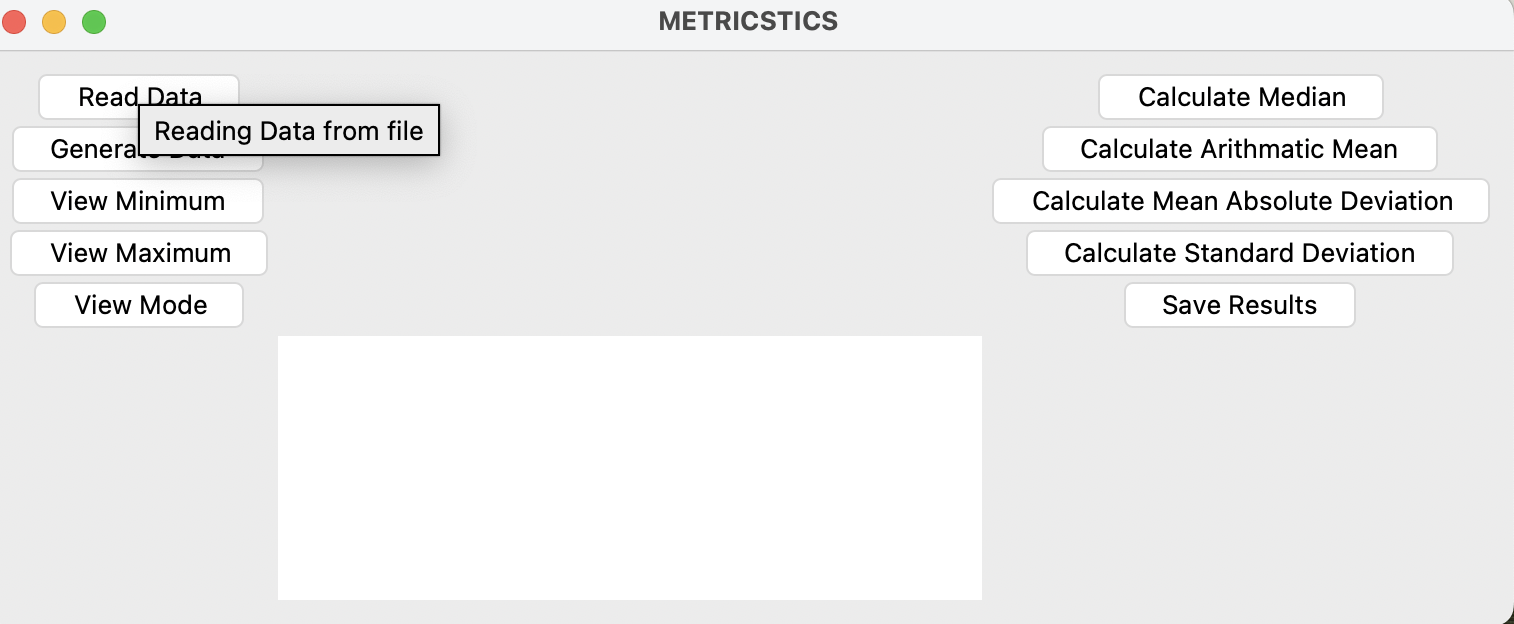
\includegraphics[width=0.9\linewidth]{ReadData.png}
        \caption{How to use Read Data functionality}
    \end{figure}
    \vspace{20em}
    \begin{figure}[h]
        \centering
        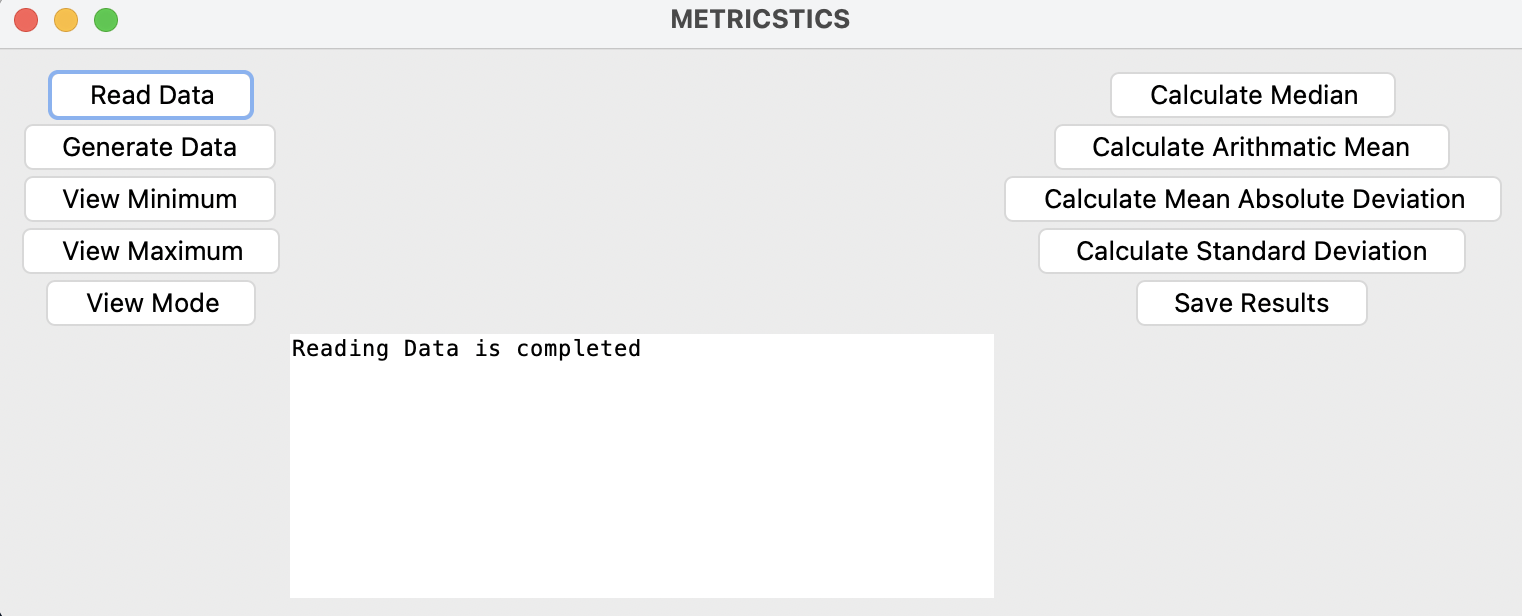
\includegraphics[width=0.9\linewidth]{ReadDataResults.png}
        \caption{Read Data Results}
    \end{figure}

    \item \textbf{Calculate Minimum:} Following screenshot shows how to use view minimum  functionality along with the results. On pressing this button, the system will give you minimum number from the list of elements (if generated using generate data or if read from file)

    \begin{figure}[h]
        \centering
        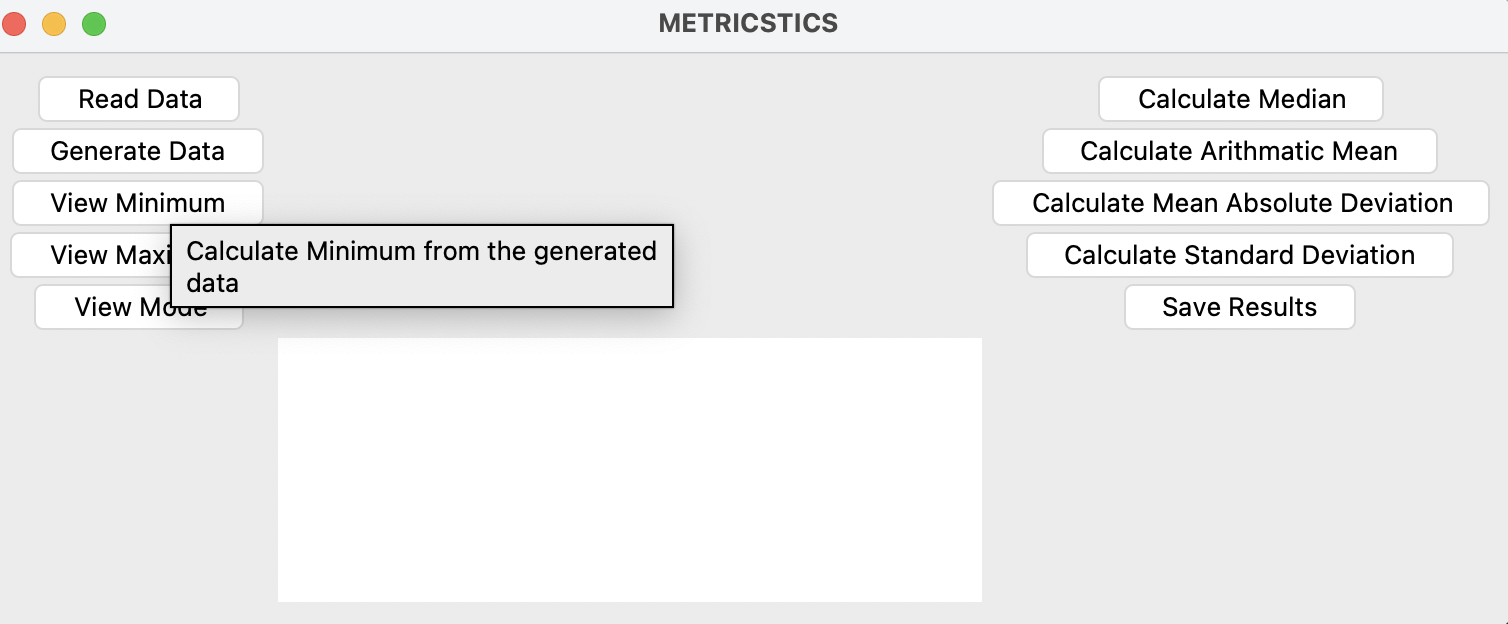
\includegraphics[width=0.9\linewidth]{ViewMinimum.png}
        \caption{How to use View Minimum functionality}
    \end{figure}
    \vspace{20em}
    \begin{figure}[h]
        \centering
        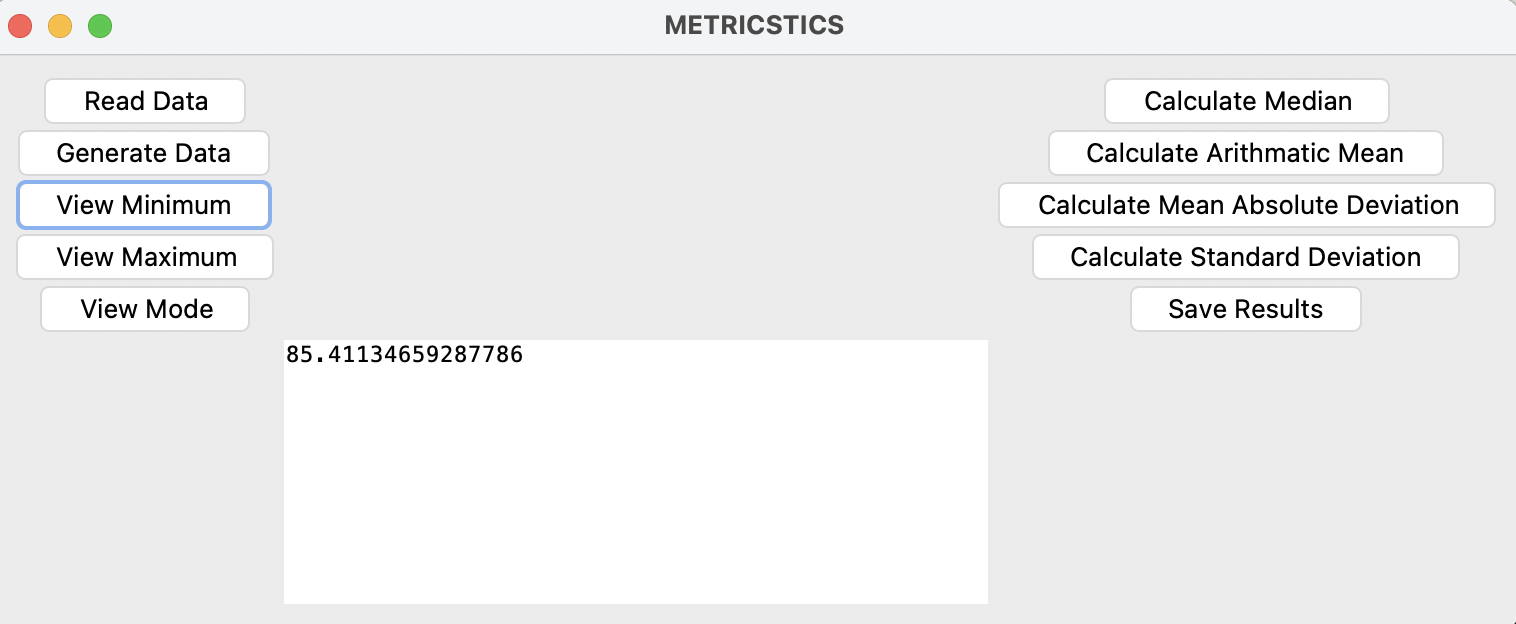
\includegraphics[width=0.9\linewidth]{ViewMinimumResults.png}
        \caption{View Minimum Results}
    \end{figure}

    \item \textbf{Calculate Maximum:} Following screenshot shows how to use view maximum  functionality along with the results. On pressing this button, the system will give you maximum number from the list of elements (if generated using generate data or if read from file)

    \begin{figure}[h]
        \centering
        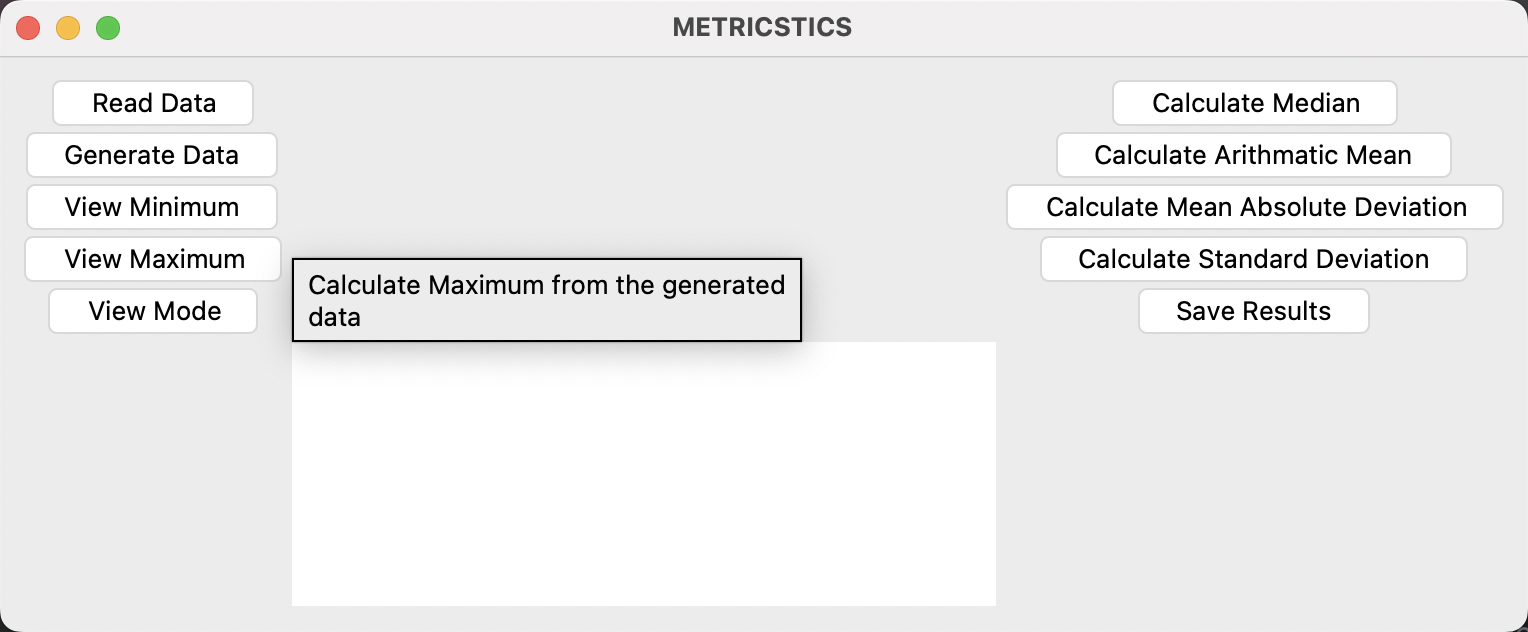
\includegraphics[width=0.9\linewidth]{ViewMaximum.png}
        \caption{How to use View Maximum functionality}
    \end{figure}
    \vspace{20em}
    \begin{figure}[h]
        \centering
        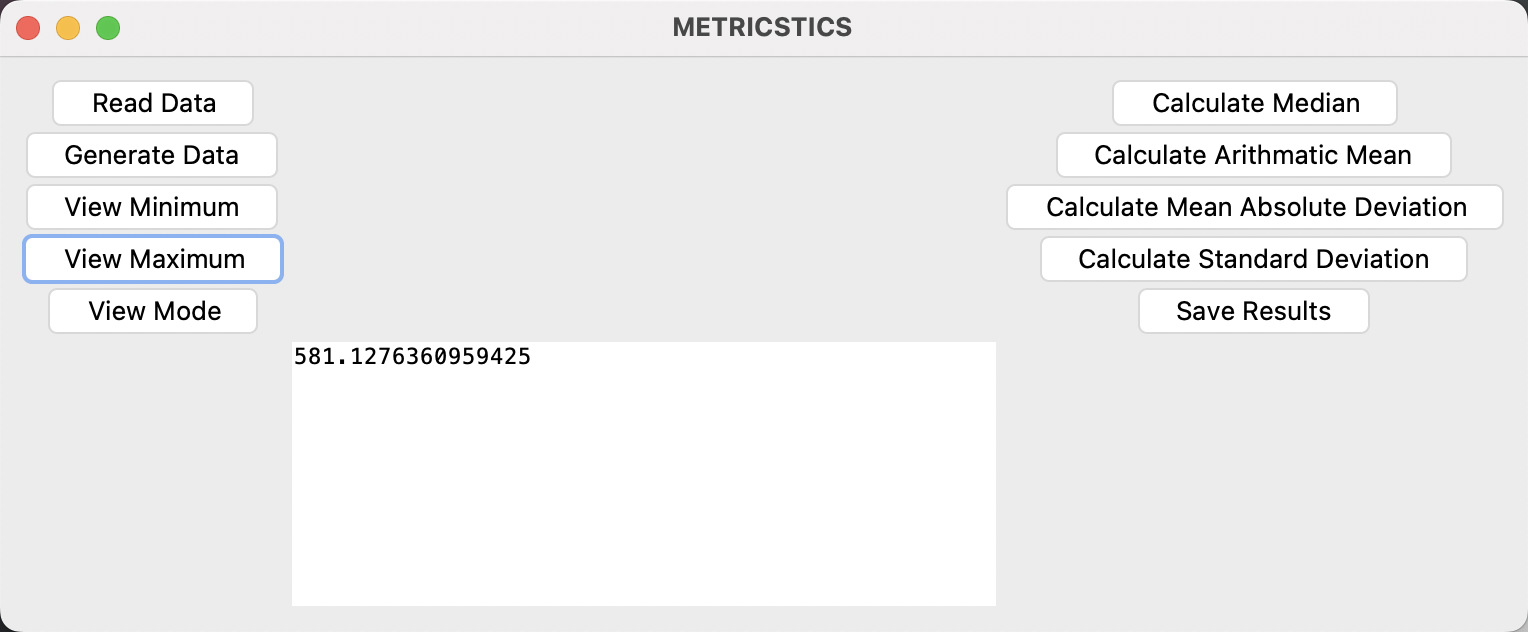
\includegraphics[width=0.9\linewidth]{ViewMaximumResult.png}
        \caption{View Maximum Results}
    \end{figure}

    \item \textbf{Generate Data:} The Following screenshot shows how to use generate data functionality along with the results.On hovering on the button the system will display a tool tip of what button does. On pressing this button, the system will display the random generated data.
    \begin{figure}[h]
        \centering
        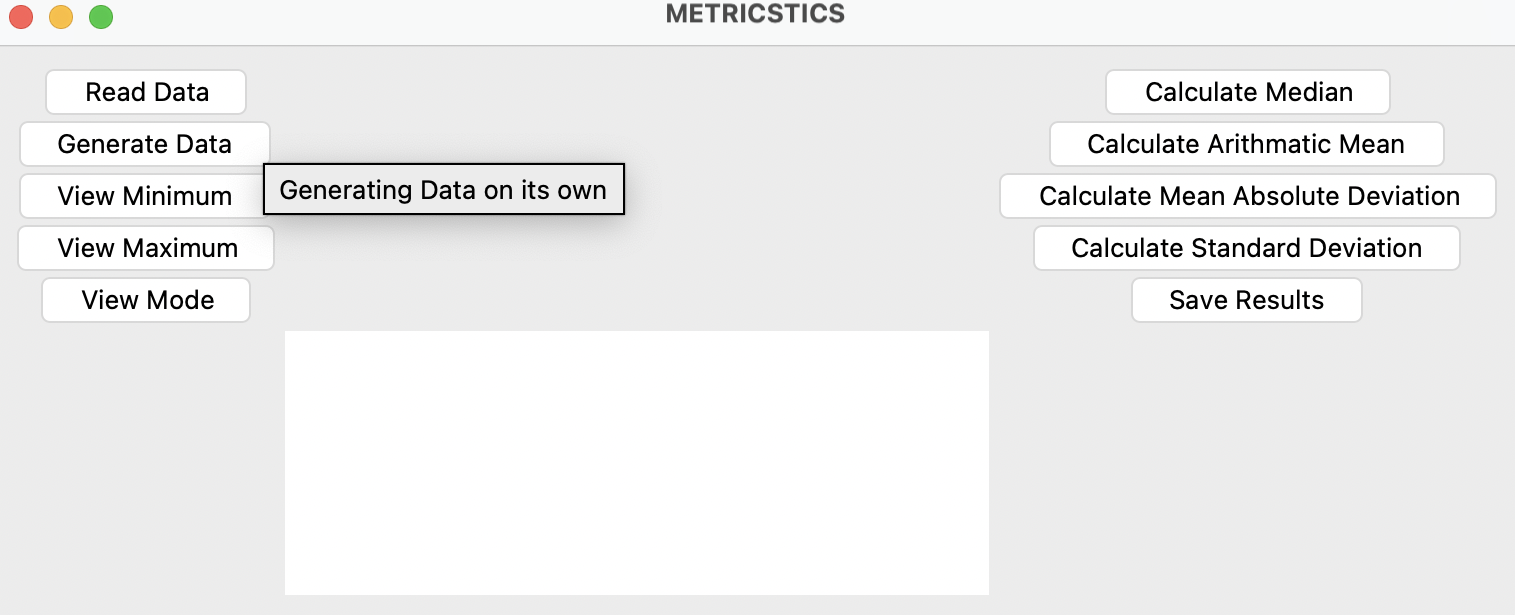
\includegraphics[width=0.9\linewidth]{GenerateData.png}
        \caption{How to use Generate Data functionality}
    \end{figure}
    \vspace{20em}
    \begin{figure}[h]
        \centering
        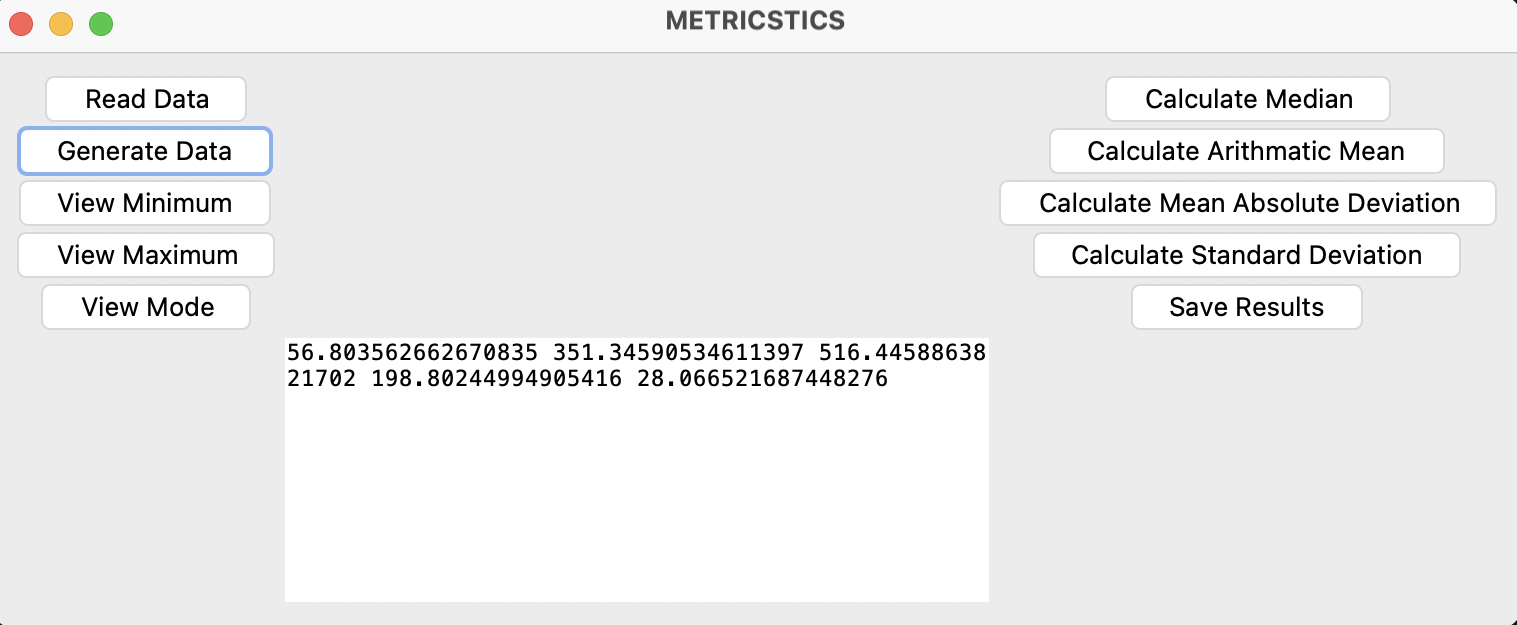
\includegraphics[width=0.9\linewidth]{GenerateDataResults.png}
        \caption{Generate Data Results}
    \end{figure}

    \item \textbf{Calculate Median:} The Following screenshot shows how to use calculate median functionality along with the results.On hovering on the button the system will display a tool tip of what button does. On pressing this button, the system will display the median of the data set.
    \begin{figure}[h]
        \centering
        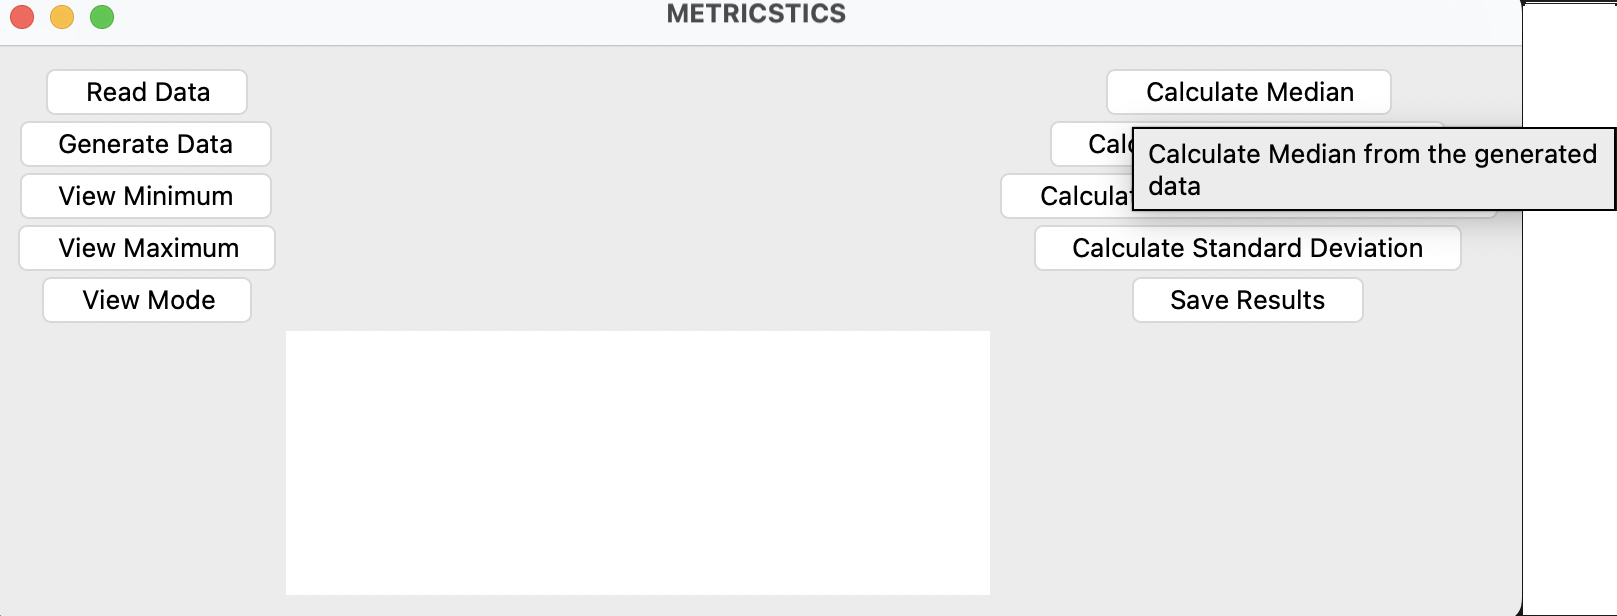
\includegraphics[width=0.9\linewidth]{Calculate Median.png}
        \caption{How to use Calculate Median functionality}
    \end{figure}
    \vspace{20em}
    \begin{figure}[h]
        \centering
        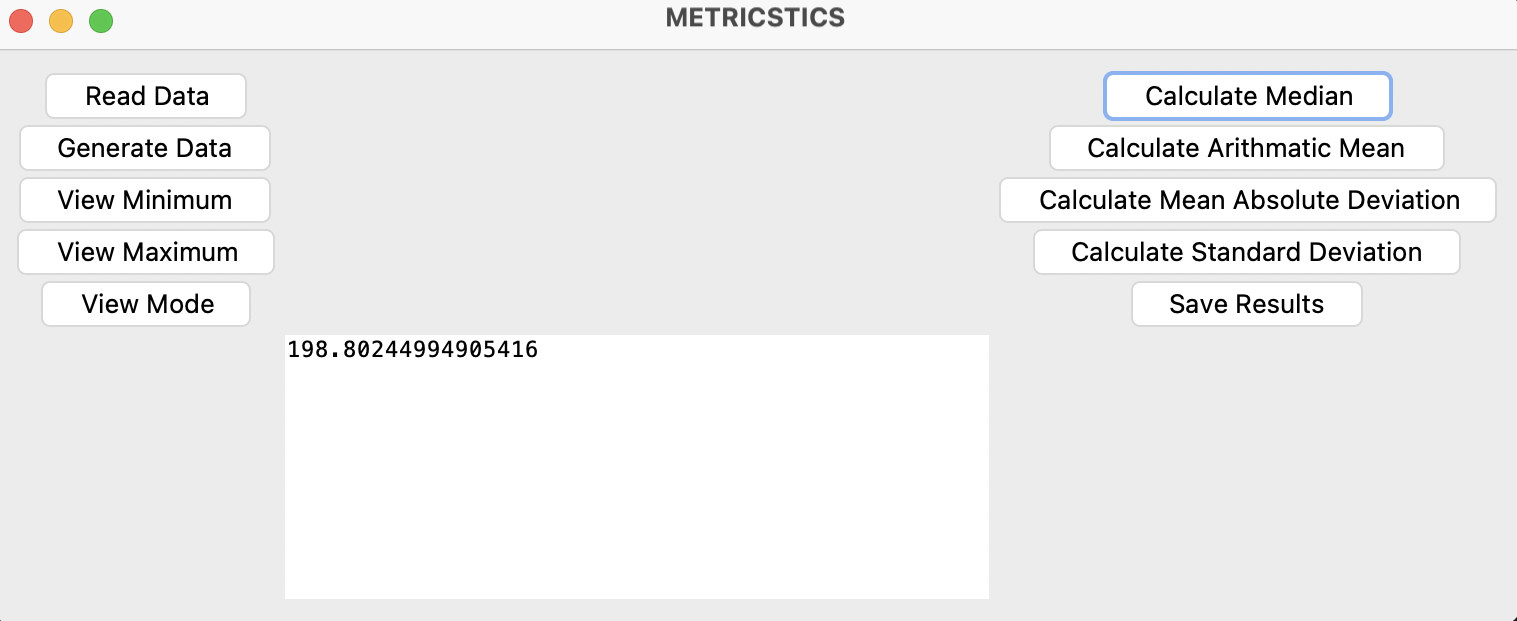
\includegraphics[width=0.9\linewidth]{CalculateMedianResults.png}
        \caption{Calculate Median Results}
    \end{figure}

    \item \textbf{Calculate Mode:} Following screenshot shows how to use view mode functionality along with the results. On pressing this button, the system will give you mode from the list of elements (if generated using generate data or if read from file)

    \begin{figure}[h]
        \centering
        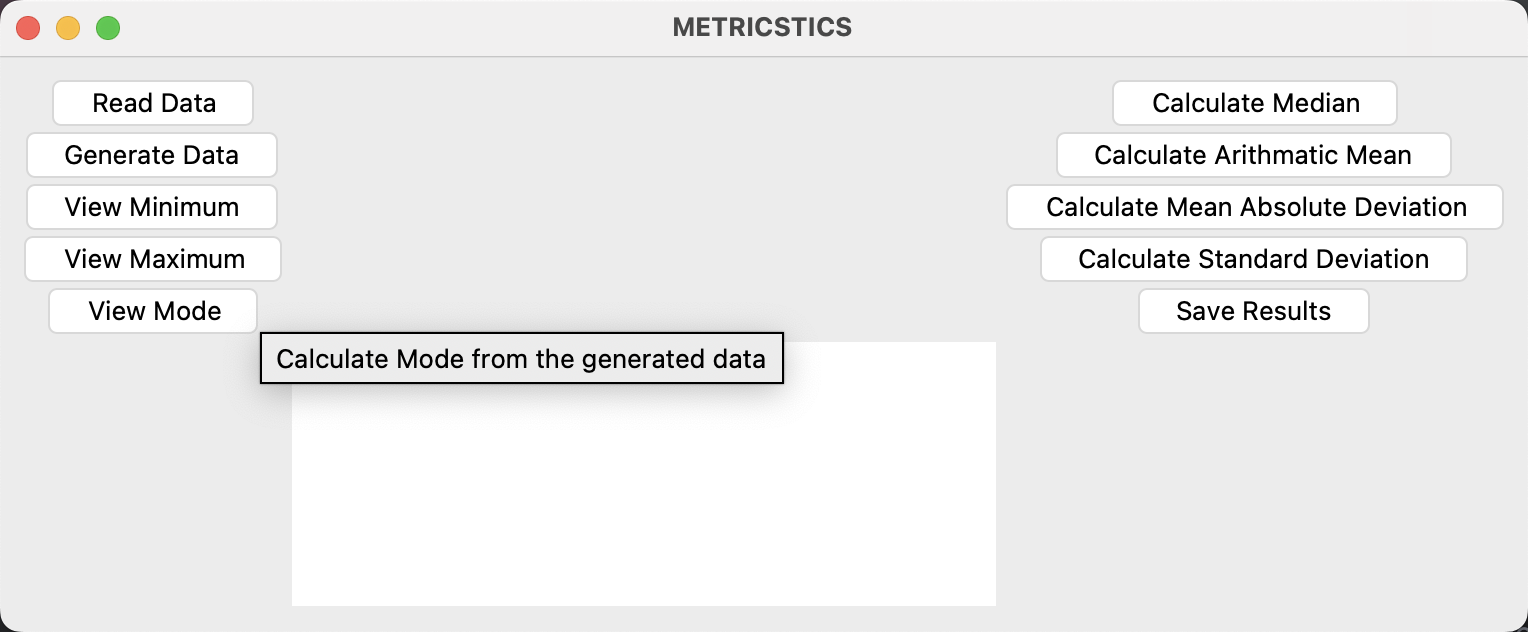
\includegraphics[width=0.9\linewidth]{ViewMode.png}
        \caption{How to use View Mode functionality}
    \end{figure}
    \vspace{20em}
    
    \begin{figure}[h]
        \centering
        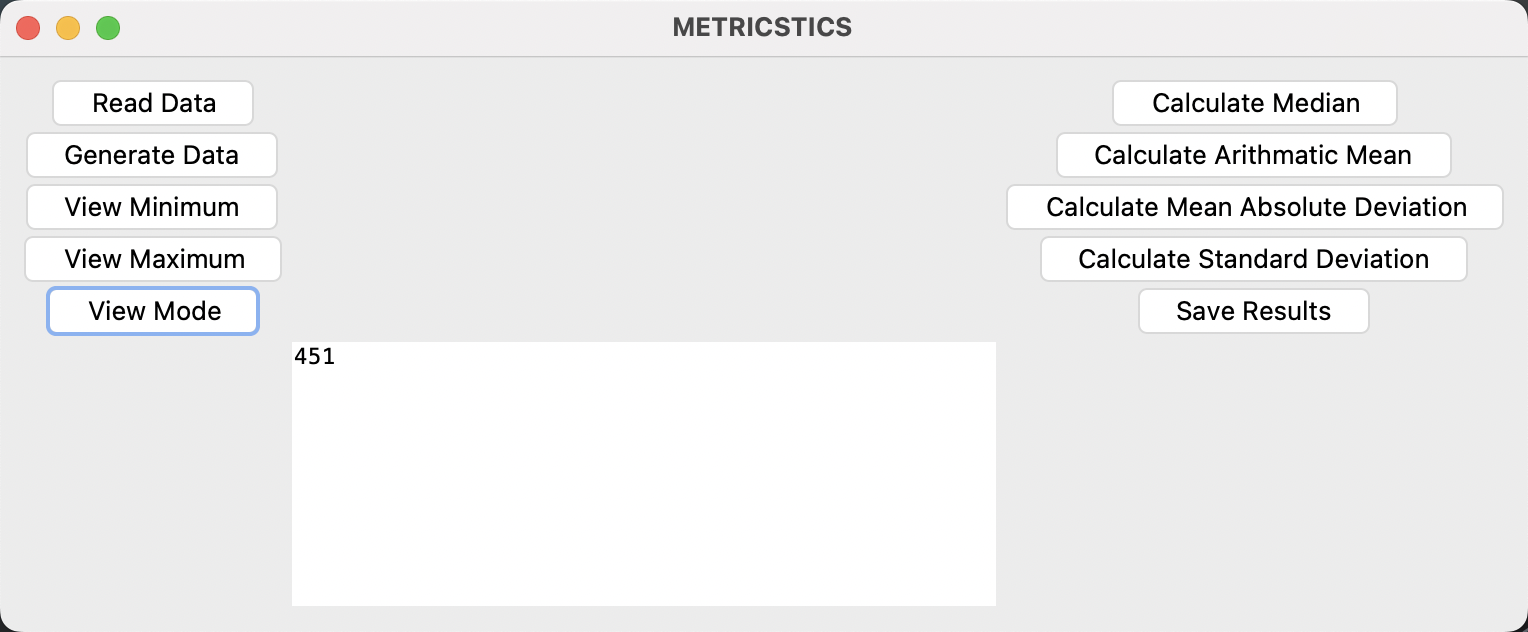
\includegraphics[width=0.9\linewidth]{ViewModeResultValid.png}
        \caption{View Mode Results}
    \end{figure}

    \item \textbf{Calculate Arithmetic Mean:} After reading or generating data, choose Calculate Arithmetic Mean. The result is displayed in the text box.

    \begin{figure}[h]
        \centering
        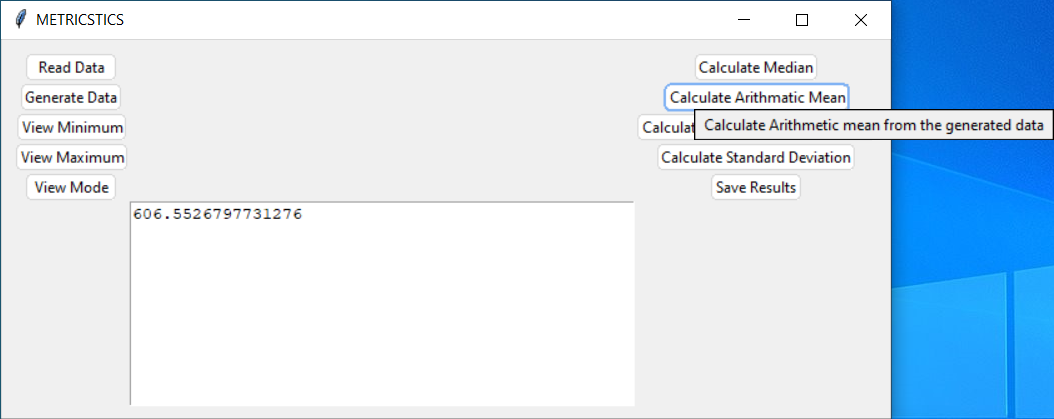
\includegraphics[width=0.9\linewidth]{CalculateArithmeticMean.png}
        \caption{How to use Calculate Arithmetic Mean}
    \end{figure}
    \vspace{20em}

    \item \textbf{Calculate Mean Absolute Deviation:} After reading or generating data, choose Calculate Mean Absolute Deviation. The result is displayed in the text box.

    \begin{figure}[h]
        \centering
        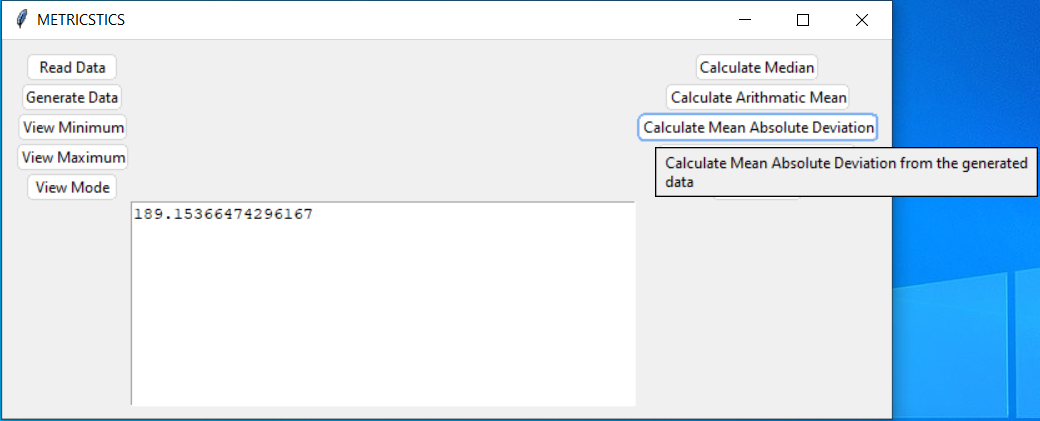
\includegraphics[width=0.9\linewidth]{CalculateMeanAbsoluteDeviation.png}
        \caption{How to use Calculate Mean Absolute Deviation}
    \end{figure}
    \vspace{20em}

    \item \textbf{Calculate Standard Deviation:} After reading or generating data, choose Calculate Standard Deviation. The result is displayed in the text box.

    \begin{figure}[h]
        \centering
        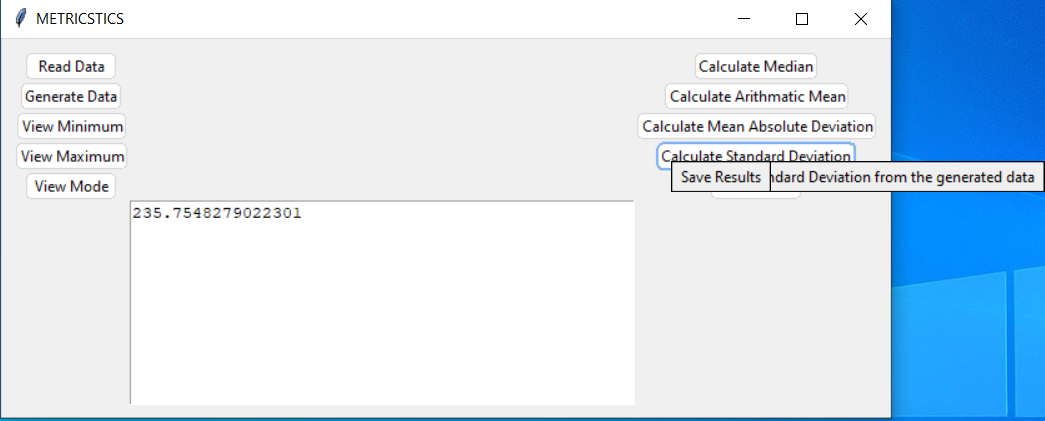
\includegraphics[width=0.9\linewidth]{CalculateStandardDeviation.png}
        \caption{How to use Calculate Standard Deviation}
    \end{figure}
    \vspace{20em}

\item \textbf{Save Button:} Following screenshot shows the functionality of save results. On pressing this button, the system will calculate all the seven calculations:  minimum ,  maximum values, median , mode, Arithmetic mean, Mean Absolute Deviation and Standard Deviation  and display the result on the view. Once it displays the result on the view it prompts for a save file dialog box and once the user saves it on their preferred directory, the file gets saved and its path is displayed on the view.




\begin{figure}[h]
        \centering
        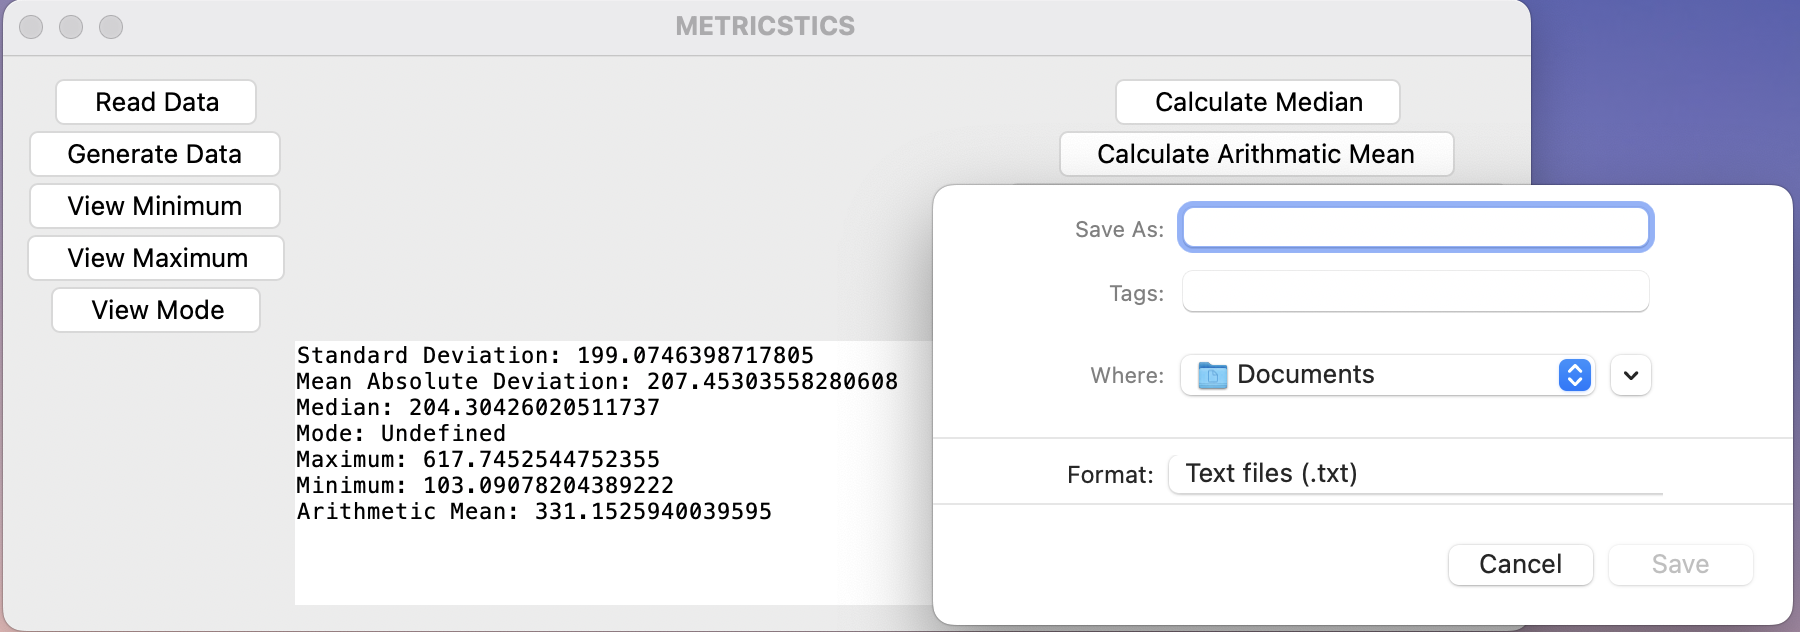
\includegraphics[width=0.9\linewidth]{Save_0.png}
        \caption{How to use Save Button functionality}
    \end{figure}
    \vspace{20em}

\begin{figure}[h]
        \centering
        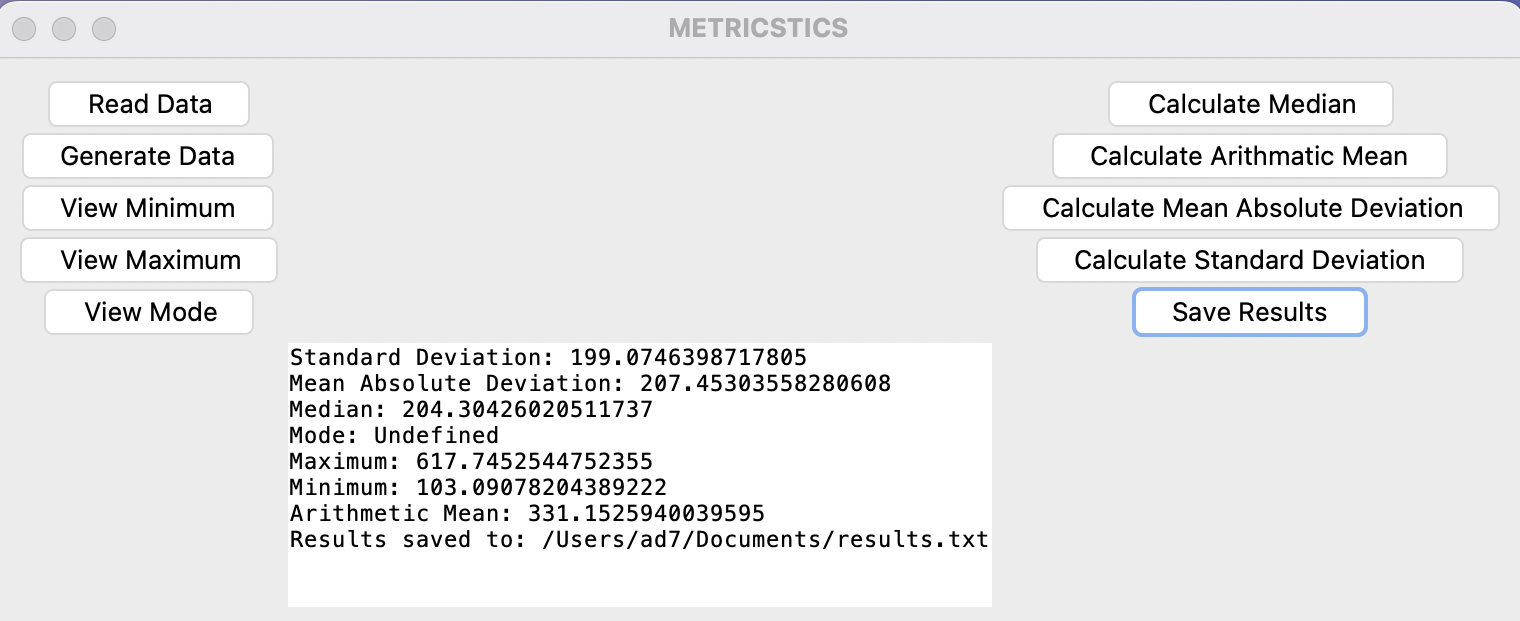
\includegraphics[width=0.9\linewidth]{Save_1.png}
        \caption{How to use Save Button functionality}
    \end{figure}
    \vspace{20em}


\end{enumerate}



\end{document}
